\section{Implementation}

\label{sec:implementation}

In this section we shall detail our implementation of the trading and peer
prediction mechanism. The system consists of five independent parts:

\begin{enumerate}
	\item Database
	\item Trading
	\item Arbitration
	\item Server
	\item User experience
\end{enumerate}

\subsection{Database}

\label{sec:database}

\subsubsection{Table Definitions}

We define three tables that handle all interactions with the database:
\code{USER}, which stores all users in the system and their remaining budget;
\code{SECURITY}, which is stores the wager, deadline, number of shares, and
final outcome for every user-created security; and \code{USER-SECURITY}, which
is responsible for the many-to-many relationship that users may have with
securities, and allows us to store user positions as well as reports once the
deadline has passed. The table definitions are as follows:

\begin{table}[ht]
	\label{tab:tableDefinitions}
	\centering
	\begin{tabular}{|c|c|c|}
		\hline
		\textbf{User} & \emph{name} & \emph{budget} \\ \hline
	\end{tabular} \\~\\

	\begin{tabular}{|c|c|c|c|c|}
		\hline
		\textbf{Security} & \emph{bet} & \emph{shares} & \emph{deadline} &
		\emph{outcome} \\ \hline
	\end{tabular} \\~\\

	\begin{tabular}{|c|c|c|c|c|c|c|}
		\hline
		\textbf{User-security} & \emph{user} & \emph{security} & \emph{shares}
		& \emph{report} & \emph{positive belief} & \emph{negative belief} \\
		\hline
	\end{tabular} \\~\\
	\caption{Table definitions in our database}
\end{table}

An entry in the \code{USER} table consists of a username and a budget. All
users currently start with \$100, which is of no real consequence since the
market uses play-money. Currently there is no requirement to supply a password
when logging in; this has been done to speed up the testing process, and if
required in the future this will be a simple addition to make.

Securities are also simple entities to store, whose fields fully describe a
market: \emph{bet} stores a string that specifies the wager being made;
\emph{shares} stores the total number of shares (referred to as $q$ in
Section~\ref{sec:tradingMechanisms}); \emph{deadline} holds the date and time
by which trading is to stop; and \emph{outcome} is initially null and
eventually set to the payout price per share, or the fraction of arbiters
reporting a positive outcome, once the deadline has passed.

The \code{USER-SECURITY} table represents the many-to-many mapping between
users and securities, and is used to store a user's position in a given market
as well as the outcome they have reported for it, if they have acted as an
arbiter. The columns are as follows: \emph{user} holds a reference to an entry
in the \code{USER} table; \emph{security} holds a reference to an entry in the
\code{SECURITY} table; \emph{shares} stores the user's position in this market
if they have one, otherwise 0; \emph{report} stores the user's report on the
outcome, if they are an arbiter for this security; and \emph{positive belief}
and \emph{negative belief} represent how reliable a user's signals are, based
on their previous reporting history. The manner in which we use the last two
fields will be discussed in greater depth in Section~\ref{sec:arbitration}.

\subsubsection{Database Interface}

We provide the interface with which we interact with the database in
\code{database.lisp}. We first initialise the database and connect to it, and
then define the tables as in the previous section. We opt to use MySQL as the
backend simply as it was already installed on the development machine, as well
as some prior familiarity with the language.  Tables are then created using the
\code{deftable} macro supplied by Mito: syntactically, this is similar to
vanilla Common Lisp's \code{defstruct} macro.  Listing~\ref{lst:deftable} shows
how we define the columns and their associated datatypes. The macro defines the
default accessors\footnote{Functions for accessing members of a struct.}, the
slots \code{created\_at} and \code{updated\_at}, and a primary key \code{id} if
none is specified. As the listing shows, we can specify a previously defined
table as the column datatype, in this case \code{user} and \code{security}, in
order to model the foreign key relation in a straightforward manner. 

\begin{lstlisting}[float,
	label={lst:deftable},
	caption={Defining the \code{USER-SECURITY} table in Mito}]
(deftable user-security ()
          ((user :col-type user)
           (security :col-type security)
           (shares :col-type :integer
                   :initform 0)
           (report :col-type (or :integer :null))
           (positive-belief :col-type (or :double :null))
           (negative-belief :col-type (or :double :null))))
\end{lstlisting}

Insertion is similarly straightforward: to insert a new entry into a table we
simply create an instance of the structure that is implicitly defined when calling
\code{deftable} then call \code{create-dao}. To retrieve records from the
database we can use either \code{select-dao} or \code{find-dao}: the former
returns all records satisfying the criteria provided, while the latter returns
the first match.

We design the interface to the database so that no custom queries need to be
created outside of \code{database.lisp}. This ensures the code interacting with
it can be kept as clean and simple as possible. We use another library from
Quicklisp, SXQL, in order to build the more complex queries to the database.
For example, Listing~\ref{lst:retrieveExpiring} shows how we retrieve all the
securities whose deadline is yet to pass, in order of first to last to expire.
We use the SXQL functions \code{where}, \code{:>}, \code{order-by}, and
\code{:asc} that expand into the corresponding MySQL code for Mito to execute.

\begin{lstlisting}[float,
	label={lst:retrieveExpiring},
	caption={Retrieving active markets using Mito and SXQL}]
(defun get-expiring-securities (datetime)
  " return all securities ordered by deadline, most imminent first "
  (with-open-database
    (select-dao 'security
                (where (:> :deadline datetime))
                (order-by (:asc :deadline)))))
\end{lstlisting}

For any interaction with the database, we need to establish a connection prior
to the transaction and disconnect after it is complete. This gives us the
opportunity to make use of Lisp's macro system: while it is a small example,
since its use is so widespread it greatly reduces the number of lines and
ensures we never forget to close a database connection. We define our macro
\code{with-open-database} as in Listing~\ref{lst:databaseMacro}. Since the
final statement in a function or macro definition in Lisp is the value returned
by that block, we are able to open the connection, execute arbitrary code and
store the final result in the variable \code{result}, then disconnect from the
database and return the result of the transaction.

\begin{lstlisting}[float,
	label={lst:databaseMacro},
	caption={Defining our \code{with-open-database} macro}]
(defmacro with-open-database (&body code)
  " execute CODE without worrying about the connection "
  `(progn
     (connect-database)
     (let ((result (progn ,@code)))
       (disconnect-database)
       result)))
\end{lstlisting}

In order to enable the transactions in the following sections, when we first
initialise the database we create a user with the name ``bank''. All money that
is then to be collected from or paid out to users is done so through this user,
so that money is largely conserved. Although not so important for a play-money
market, it does help for accounting purposes.

\subsection{Trading}

\label{sec:trading}

Trading allows us to gather public sentiment on the user-defined securities,
and this part of the system is responsible for setting share prices,
calculating the cost of transactions, and charging fees to raise funds for the
arbitration stage, to ensure arbiters are incentivised to report truthfully.
These features are implemented in the files \code{msr.lisp} and
\code{market.lisp}.

We implement our automated market maker using a scoring rule market.  In order
to achieve the guarantees of Freeman, Lahaie, and Pennock's mechanism we must
use a scoring rule that is strictly proper, which can then be implemented as a
market maker based on a convex cost function. We use the commonly-used
Logarithmic Market Scoring Rule (LMSR) created by Robin
Hanson~\cite{Hanson2007}, whose cost function is defined as follows:
%
\begin{equation}
	\label{eq:LMSR}
	C(\vect{q}) = b \log \left( \sum_j e^{q_j/b} \right)
\end{equation}
%
This assumes that each security $j$ is one of a collection of mutually
exclusive and exhaustive outcomes. Since we are only dealing with binary
events, we can compute a share price based only on the number of shares bought
for the positive outcome, and assume that buying shares in the negative outcome
is equivalent to selling shares in the positive outcome. In this case, we have
$\vect{q}=( 0 , \, q_1 - q_0 )$, where $q_0$ and $q_1$ are the quantity of
shares bought by agents in the negative and positive outcomes, respectively.
This gives us the following cost function for LMSR in the binary setting, where
$q=q_1-q_0$:
%
\begin{equation}
	\label{eq:LMSRbinary}
	C_b (q) = b \log (1 + e^{q/b})
\end{equation}
%
In these cost functions, $b>0$ appears as a parameter that allows us to control
the responsiveness of $C$. A lower value of $b$ corresponds to a more sensitive
share price, meaning the price will change more quickly for smaller
transactions. It also controls the market's risk of loss: for markets with
$|\Omega|$ outcomes it can be shown that the maximum loss incurred by the
market maker is $b \log |\Omega|$. In our case, each market will lose at most
$b \log 2$. Recall that to compute the actual cost to charge an agent for a
transaction, we compute $C_b(q')-C_b(q)$ for an agent wishing to take the total
quantity of shares from $q$ to $q'$, and this also encodes sell transactions.
The share price function is the derivative of the cost function, which is in
our case:
%
\begin{equation}
	\label{eq:LMSRprice}
	p_b(q) = \frac{e^{q/b}}{1+e^{q/b}}
\end{equation}
%
Upon market creation a user is only given the option to buy a positive number
of shares -- otherwise, it would make more sense for the user to create a
market for the opposite outcome. After this, the custom security is created and
is open for all other users to trade in. The share price reflects the strength
of the community's opinion on the event's outcome: for example, at $q=0$ then
the community is exactly split on whether the event will have a positive
outcome, and appropriately $p_b(0)=\$0.50$ for any $b$. Meanwhile, for $q=20$
and $b=10$ this means twenty more shares have been bought than sold in the
market and would yield a quoted share price of $p_{10}(20) \approx \$0.88$.
Users feel more confident that the event will be positive, thus pushing the
price upwards. Suppose that upon seeing this price increase, an agent wishes to
buy ten more shares in the market: they would then be required to pay
$C_{10}(30)-C_{10}(20)=10 \log (\frac{1+e^3}{1+e^2}) \approx \$9.22$. Such an
action in the market would push the share price to $p(30) \approx \$0.95$, plus
any fees. Figure~\ref{fig:marketCreation} shows the interface for creating a
new market, while Figure~\ref{fig:transactionSummary} shows an example of the
transaction summary that a user is presented with after having done so.

\begin{figure}[h]
	\centering
	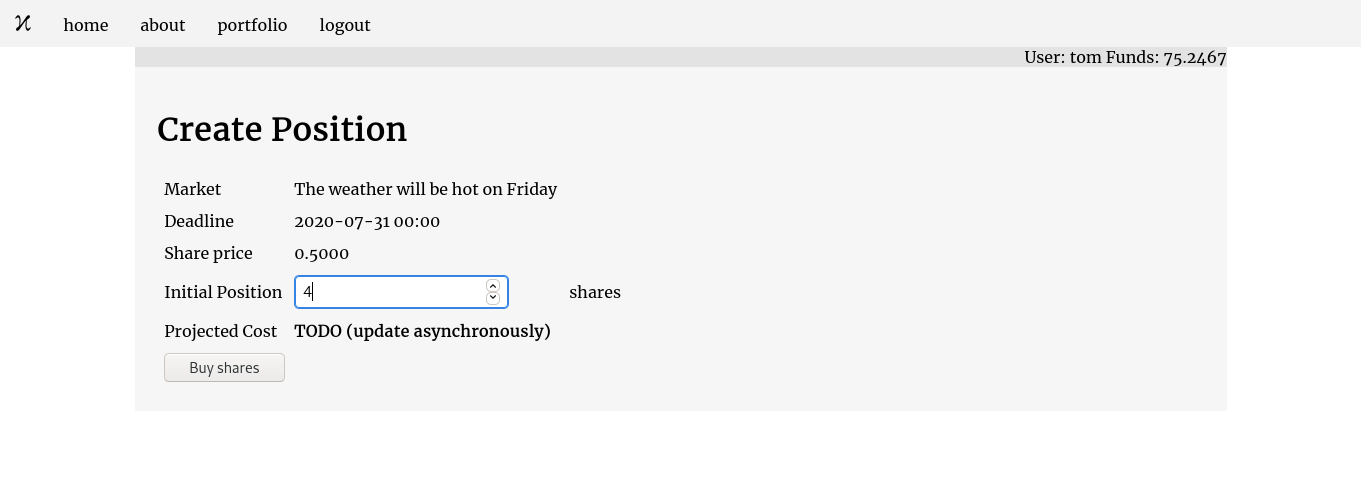
\includegraphics[width=\textwidth]{market-creation}
	\caption{The interface for creating a new market}
	\label{fig:marketCreation}
\end{figure}

\begin{figure}[h]
	\centering
	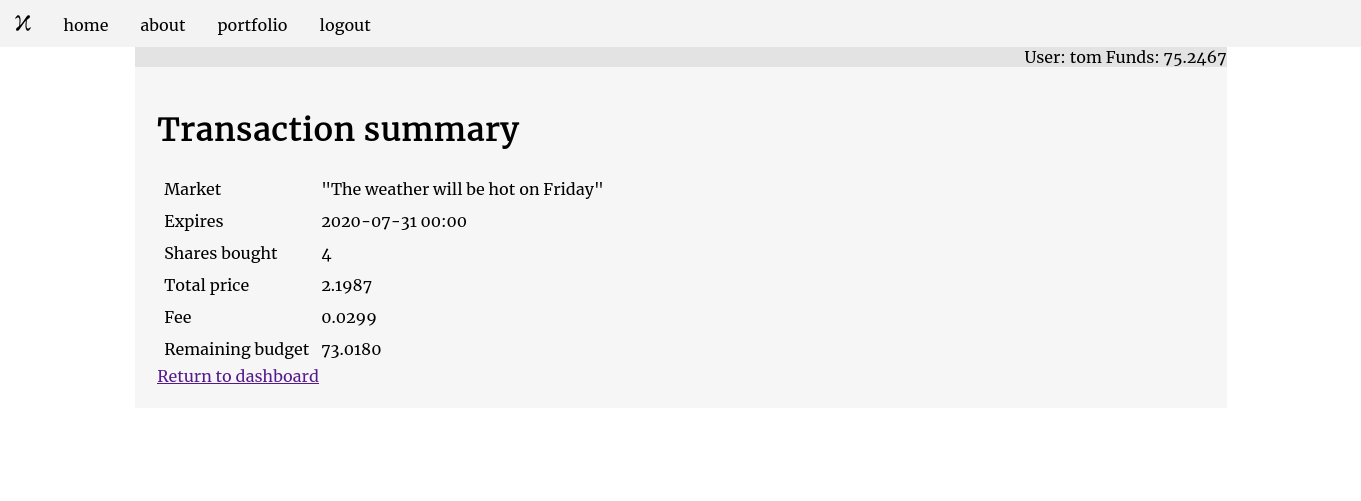
\includegraphics[width=\textwidth]{transaction-summary}
	\caption{Users are presented with a transaction summary upon creating a new
	market}
	\label{fig:transactionSummary}
\end{figure}

Fees are only charged on transactions where an agent increases their risk: this
means they are buying or selling a greater number of shares than their current
position. For example, a user owning ten shares and selling five would incur no
extra cost since they are liquidating a position they have already invested in,
while selling more than ten or buying additional shares would incur an
additional cost. The fee serves a secondary purpose in bounding the price of
the security away from \$0 and \$1, as a potential trader would be spending
more than \$1 or less than \$0 to buy or sell the shares. For example, even if
an agent were to buy an infinitesimal number of shares, meaning their
transaction cost would be given by the share price function $p$, if the share
price was \$0.99 and the transaction fee was set to 5\%, they would be required
to pay $\$0.99 \cdot 1.05 = 1.0395$, greater than the maximum possible payout.
This allows us to bound the total number of securities that will exist for a
given market, and hence its maximum payout.  In our market we implement a fixed
trading fee of 5\% on all risk transactions.

Obviously, we need to take into account a trader's budget when they are looking
to make a transaction and if they cannot afford one, deny them the trade. This
is simple for buy transactions, where the cost must not exceed their budget.
For a short sell, we need to ensure that the user will be able to cover the
expense of buying back the shares in the worst case -- that is, the event
occurs and they are required to buy back their position at \$1 per share. Hence
the function, \code{sufficient-funds?}, ensures a user can only go short on a
security if their budget plus the amount they are paid for shorting is larger
than the size of their short position.

\begin{figure}[h]
	\centering
	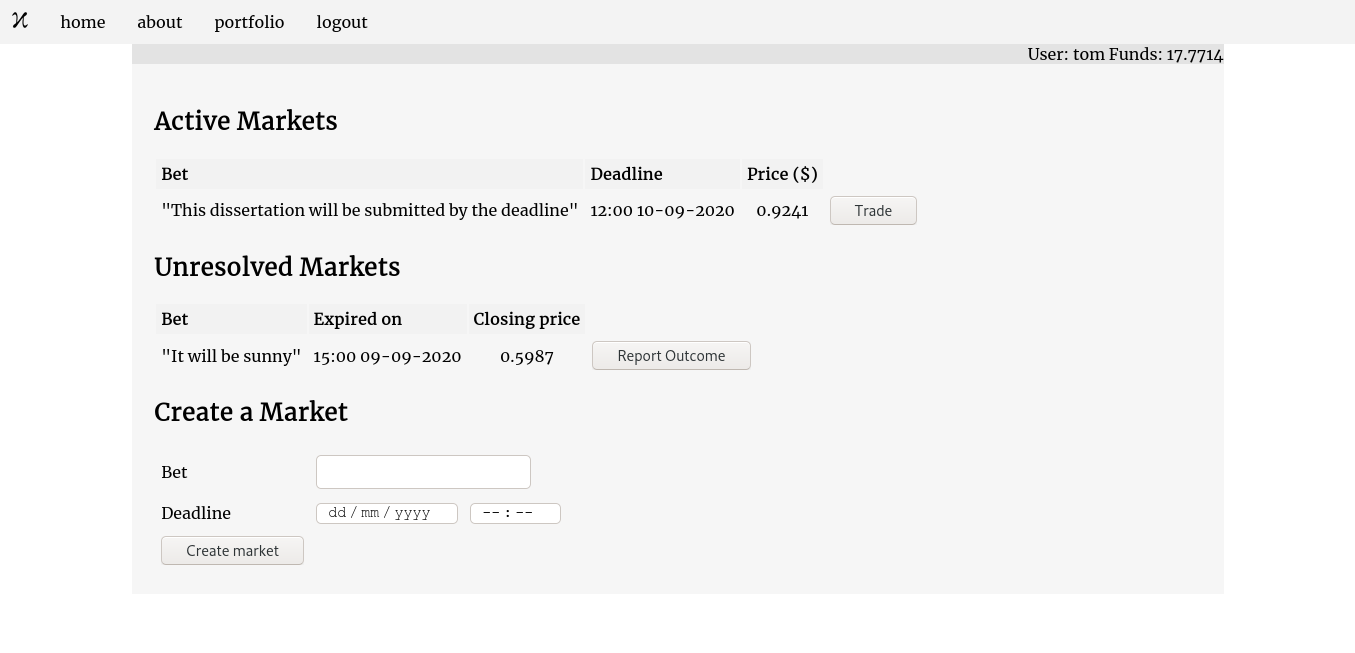
\includegraphics[width=\textwidth]{trade}
	\caption{Users can trade in active markets or report on those that have
	expired}
	\label{fig:trade}
\end{figure}

\subsection{Arbitration}

\label{sec:arbitration}

\subsubsection{Computing signal reliability}

The arbitration stage is where we resolve market outcomes using arbiter reports
and pay out winnings to, or demand payment from, stakeholders in the security.
Since the mechanism incentivises arbiters to act truthfully even if an arbiter
themselves holds a stake in the market, we decide to let anyone opt in to
reporting on the outcome. Once a market's deadline has passed the security will
be listed as an expired market and the user is presented with the option to act
as an arbiter, as in Figure~\ref{fig:trade} under ``Unresolved Markets''. After
doing so, they may then input their observed signal, or indeed a lie, as
Figure~\ref{fig:reportOutcome} shows. Once the required number of reports have
been collected, we move onto rewarding arbiters for submitting reports and
computing the final outcome of the market.

\begin{figure}[h]
	\centering
	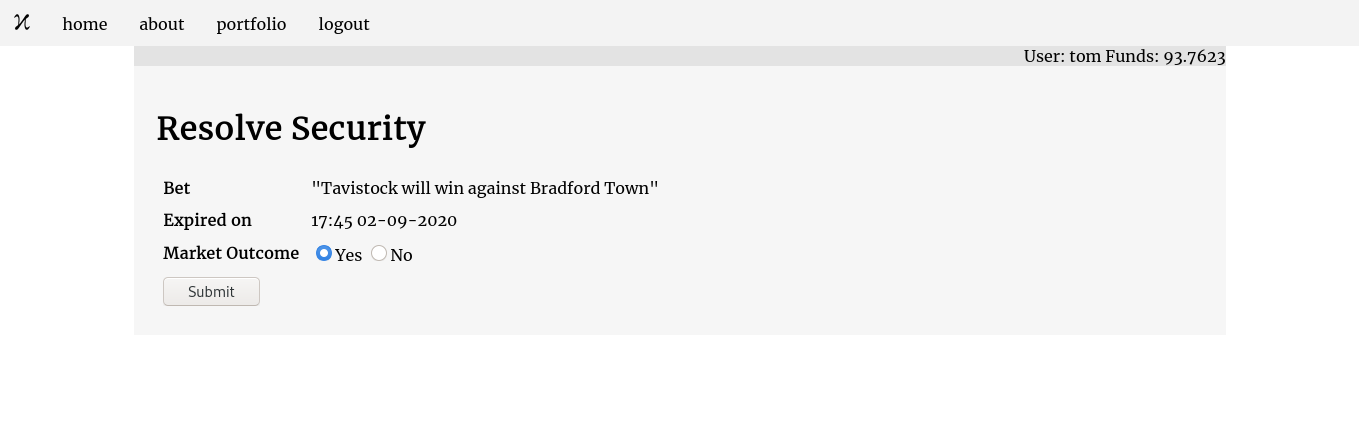
\includegraphics[width=\textwidth]{report-outcome}
	\caption{The interface by which arbiters report market outcomes}
	\label{fig:reportOutcome}
\end{figure}

%\begin{figure}[h]
%	\centering
%	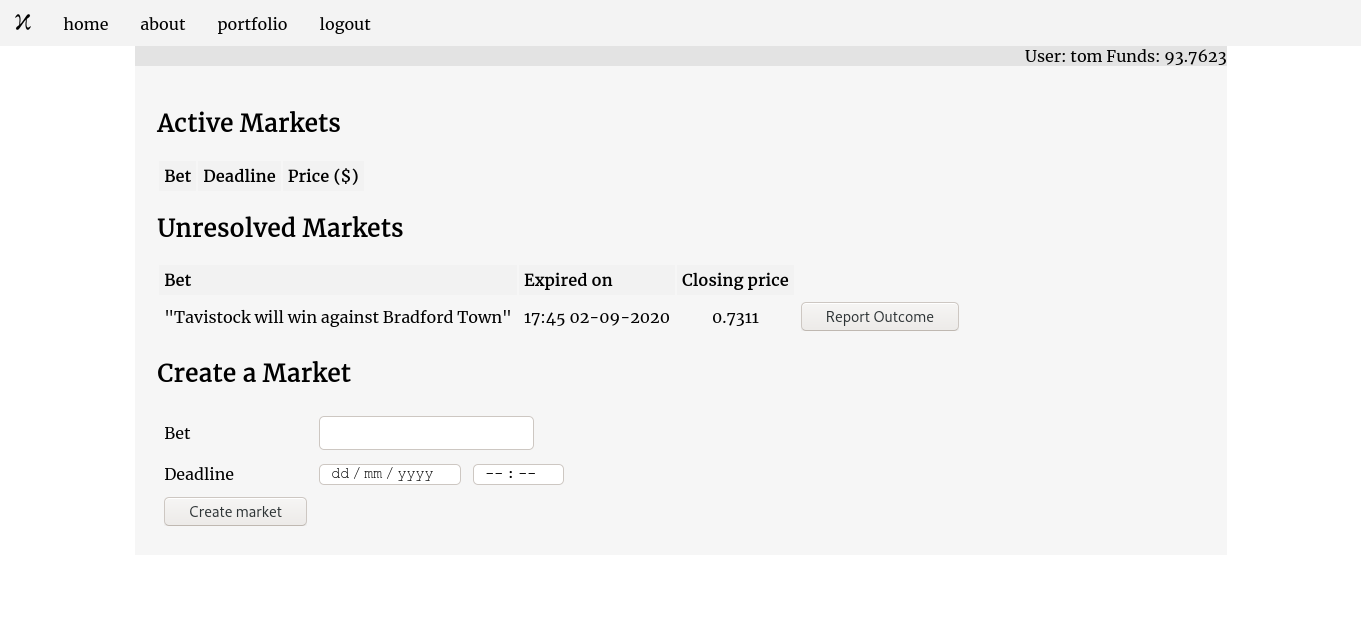
\includegraphics[width=\textwidth]{expired-market}
%	\caption{Users may opt in to report on market outcomes}
%	\label{fig:expiredMarket}
%\end{figure}

Arbiters are rewarded by being paid a certain amount of money only if their
report agrees with that of another randomly chosen arbiter. The reward is
determined by the 1/prior-with-midpoint mechanism, where instead of using the
common prior probability $\mu$ we use the update probabilities $\mu_1$ and
$\mu_0$. Recall that these are the probability that, given that arbiter $i$
receives a positive signal, so too does another randomly chosen arbiter $j$,
and the probability that, given that $i$ receives a negative signal, another
randomly chosen arbiter $j$ receives a positive signal. Since we cannot assume
arbiters to act truthfully, this is more complicated than simply counting the
types of reports received. Instead, we use information about signal error rates
$\Pr[x_i=1|X=1]$ and $\Pr[x_i=1|X=0]$ based on past market outcomes and past
reporting behaviour for each arbiter $i$. This is a fairly involved process:
first we gather all securities that have been reported on in the past by $i$
and whose outcome has been determined; we then iterate through each one of
these returned securities and determine the report that $i$ submitted as well
as its outcome, and push this into a list of results. At the end of this stage
we have a list \code{((security report outcome) ...)} that describes the
arbiter's report and the market's true (peer-determined) outcome for each
security for which they have acted as an arbiter. The code implementing this is
shown in Listing~\ref{lst:reportingHistory}.

\begin{lstlisting}[float,
	label={lst:reportingHistory},
	caption={Gathering a user's reporting history}]
(defun get-securities-reported-by-user (user)
  (with-open-database
    (select-dao 'security (inner-join 'user-security
                                      :on (:= :security.id
                                              :user-security.security-id))
                (where (:and (:= :user-security.user-id (user-id user))
                             (:not-null :security.outcome)
                             (:not-null :user-security.report))))))

(defun get-reporting-history (user)
  (let ((securities (get-securities-reported-by-user user))
        security-reports)
	(dolist (security securities)
	  (with-open-database
	    (let ((report (user-security-report
	                    (find-dao 'user-security
	                              :user user
	                              :security security)))
              (outcome (security-outcome security)))
	      (if outcome
            (push (list security report outcome) security-reports)))))
	security-reports))
\end{lstlisting}

We then use this history to compute the probability that, assuming the arbiter
has always acted truthfully, their signal has been correct in telling them the
true outcome of the event. We refer to these probabilities, $\Pr[x_i=1|X=1]$
and $\Pr[x_i=1|X=0]$, as a arbiter $i$'s positive and negative signal beliefs
as a remnant of a previous implementation. Listing~\ref{lst:positiveBelief}
shows how we calculate an arbiter's positive belief, with a similar method
applying for computing the negative belief: for the arbiter's history
restricted to the securities whose outcome was reported as positive by the
majority of arbiters, we count the number of times this arbiter also reported a
positive outcome, thus giving us the arbiter's signal error probability given
we know the outcome is (more likely to have been) positive. If there have been
no positive outcomes, then we assume the arbiter has a perfect signal.
Calculating the negative signal belief is done in a similar manner: first we
collect items of the arbiter's reporting history where the security was mostly
reported as a negative outcome, then we count the number of times this arbiter
submitted a positive report. Again we assume in the lack of markets with
negative outcomes that the arbiter has a perfect signal. We repeat this to
compute the positive and negative signal beliefs for each arbiter.

\begin{lstlisting}[float,
	label={lst:positiveBelief},
	caption={Computing an arbiter's positive signal belief given
	their reporting history}]
(defun calculate-positive-belief (reporting-history)
  ;; first only get the reports where the outcome was positive
  (let ((positive-outcomes (remove-if-not #'(lambda (x) (>= 0.5 (third x)))
                                          reporting-history))
        positive-reports)

    ;; now count the number of times the user reported a positive outcome
    (setf positive-reports (count T (mapcar #'(lambda (x) (equal 1 (second x)))
                                            positive-outcomes)))
    (if positive-outcomes
      (/ positive-reports (length positive-outcomes))
      1)))
\end{lstlisting}

We use this information about the reliability of each arbiter's signal, along
with the prior probability $\mu$ that the event had a positive outcome, to
compute the update probabilities $\mu_1$ and $\mu_0$, used in the
1/prior-with-midpoint mechanism. We first compute the update
probabilities $\mu_1^i$ for each arbiter $i$, using a randomly chosen peer
arbiter $j$, as follows:
%
\begin{equation}
	\label{eq:updateProbabilities}
	\begin{aligned}
		\mu_1^i & = \Pr[x_j=1|x_i=1] \\
		& = \Pr[x_j=1|X=0] \cdot \Pr[X=0|x_i=1] + \Pr[x_j=1|X=1] \cdot
		\Pr[X=1|x_i=1]
	\end{aligned}
\end{equation}
%
We use the same approach to compute $\mu_0^i$ for each $i$. The final values of
$\mu_1$ and $\mu_0$ are then calculated by taking the minimum and maximum
across all $\mu_1^i$ and $\mu_0^i$, respectively. Thus we have common update
probabilities across all agents.

\subsubsection{Rewarding the arbiters}

We may now pair arbiters randomly to pay them via the 1/prior-with-midpoint
mechanism. We first retrieve two lists from the database: the first is the list
of all arbiter reports and is of the form \code{arbiter-reports = ((arbiter
report) ...)}; the second is a list of all arbiter signal beliefs and is of the
form \code{arbiter-beliefs = ((arbiter positive-belief negative-belief) ...)}.
Since we will be pairing arbiters randomly and still need efficient access to
these values, we then create two hash tables associating an arbiter to their
report and their beliefs, giving us \code{report[i] = report} and
\code{beliefs[i] = (positive-belief negative-belief)} for each $i$. The
market's outcome is simply set to the proportion of arbiters that reported a
positive outcome. At this point we pay out the appropriate winnings to
stakeholders, paying out money to those who hold shares and demanding money
from those who have gone short. Now that the market's outcome has been
determined it will no longer be listed as an unresolved market on the user's
dashboard.

\begin{lstlisting}[float,
	label={lst:marketOutcome},
	caption={Computing the market outcome}]
(let ((reports (mapcar #'second arbiter-reports)))
  ;; the payoff of each share held is the fraction of arbiters reporting 1
  (setf outcome (float (/ (count 1 reports) (length reports)))))
\end{lstlisting}

We next compute the random pairing of arbiters. Lisp has no function to shuffle
a list, so we implement the Fisher-Yates
algorithm~\cite[pg.~26-27]{FisherYates1938} ourselves as the \code{shuffle}
function in Listing~\ref{lst:randomPairing}. The random pairing is then formed
by walking through the shuffled list and collecting adjacent elements as pairs.

\begin{lstlisting}[float,
	label={lst:randomPairing},
	caption={Assigning arbiters to peers randomly}]
(defun shuffle (lst)
  " shuffle LST randomly (without modifying it) "
  (let ((lst (copy-list lst)))
    (loop for i from (length lst) downto 2 do
          (rotatef (elt lst (random i))
                   (elt lst (1- i))))
    lst))

(defun random-pairing (lst)
  " randomly pair items from LST together if length(lst) is even "
  (if (evenp (length lst))
    (loop for (a b) on (shuffle lst) by #'cddr while b
          collect (list a b))))
\end{lstlisting}

For each set of paired arbiters we then retrieve their reports and signal
beliefs from the hash tables and compute, for each arbiter $i$ in the pair, the
values of $\mu_1^i$ and $\mu_0^i$ according to
equation~\eqref{eq:updateProbabilities}, where the randomly chosen $j$ is
simply the partner with whom they have been paired. We push these values to a
list so we may then compute the minimum value of $\mu_1^i$ and maximum value of
$\mu_0^i$ across all arbiters. Finally, to compute the smallest $k$ to satisfy
inequality~\eqref{eq:kBoundN} we set $k = \max_i 2|n_i|/m\delta$, and use this
to pay arbiters according to equation~\eqref{eq:oneOverPrior}.

\subsection{Server}

\label{sec:server}

The code from each of the separate areas of the market is then drawn together
in the file \code{server.lisp}, in which we set up the web server, define the
webpages, and call the functions from the different interfaces we provide.

We use Hunchentoot to host the web server. At startup this involves creating an
instance of a Hunchentoot \code{easy-acceptor}, which opens up a port of our
choosing to accept requests. Doing so also initialises the dispatch table,
which is a list containing the functions to execute when the corresponding
webpage is loaded. We can specify webpages to the dispatch table by using
Hunchentoot's \code{create-prefix-dispatcher} function: this simply takes a URL
and the function to execute when that URL is loaded. Again the opportunity to
use Lisp's macro system arises: the code in Listing~\ref{lst:defineURL} shows a
macro that defines a function and a URL of the same name, creates a dispatcher
for them and pushes it to the dispatch table. This again not only saves
rewriting repetitive code but also keeps the codebase clear -- for example, the
URL \code{/index} is served by a function called \code{index}. Now each time we
wish to define a new webpage we need only to call \code{define-url-fn} followed
by the name of the page and the code to execute.

\begin{lstlisting}[float,
	label={lst:defineURL},
	caption={Macroising URL functions}]
(defmacro define-url-fn ((name) &body body)
  " creates handler NAME and pushes it to *DISPATCH-TABLE* "
  `(progn
     ;; define the handler
     (defun ,name ()
       ,@body)

     ;; add the handler to the dispatch table
     (push (create-prefix-dispatcher
             ,(format NIL "/~(~A~)" name) ',name)
           *dispatch-table*)))
\end{lstlisting}

We use CL-WHO to define the content of the webpages, which translates Lisp
statements into strings of HTML. In order to achieve a consistent style while
avoiding code duplication we define a macro describing a ``standard page'', an
abridged version of which is given in Listing~\ref{lst:standardPage}. This
allows us to concisely define webpages with a similar look and feel, and only
requires us to specify the content that makes the page unique via the
\code{body} parameter.

\begin{lstlisting}[float,
	label={lst:standardPage},
	caption={Macroising webpage definitions}]
(defmacro standard-page ((&key title) &body body)
  " template for a standard webpage "
  `(with-html-output-to-string
     (*standard-output* NIL :prologue T :indent T)
     (:html :xml\:lang "en"
            :lang "en
            (:head (:title title)
                   (:link :href "/style.css" :type "text/css" :rel "stylesheet")
                   ;; rest of preamble ... )
            (:body
              (:ul :id "navbar"
                   (:li ... ))
              (:div :class "container"
                    ...
                    (:div :class "content"
                          ,@body))))))
\end{lstlisting}

Hunchentoot also automatically provides session handling -- this is obviously
important for allowing multiple users to be logged on at the same time and
presenting the appropriate information to them. All we need to do is define the
symbol \code{session-user} in the data structure for session handling, then
when a user logs in we set this value to the matching user retrieved from the
database with \code{(session-value 'session-user)}. This allows us to display
consistent user information across different webpages within the same session,
such as the user's budget or their portfolio of securities. Finally, users
mostly interact with the market through forms: Hunchentoot provides the
\code{get-parameter}, \code{post-parameter}, and \code{parameter} functions to
retrieve the values from these forms and send them to and from the different
webpages.

% session handling
% sending data e.g. (parameter ...)

\subsection{User Experience}

\label{sec:user-experience}

In Sections~\ref{sec:database}, \ref{sec:trading}, \ref{sec:arbitration}, and
\ref{sec:server} we have detailed the manner in which we achieve the goals laid
out in Section~\ref{enm:goals} which implement the core features of any
prediction market, as well as the behaviour that makes the peer prediction
mechanism of Freeman et al.\ unique. In this section we shall detail how we
make our prediction market more user-friendly and intuitive to use.

The most important aspect behind making the web application responsive is the
integration of asynchronous server communications so that we can display
up-to-date information to the user without a page refresh, as well as trigger
markets to close trading at the correct time. For this we use the Quicklisp
libraries Parenscript coupled with Smackjack to translate Lisp code to
JavaScript and allow us to communicate asynchronously with the server. We first
use Parenscript for form validation on the client-side, and in particular to
ensure that all required form fields are completed without needing to send the
entire form to the server, only for it to potentially be incomplete.
Parenscript provides the function \code{ps-inline}, which allows us to insert
Lisp code, that will be converted to a valid JavaScript program, within the
CL-WHO defined pages. We can therefore validate forms before being sent to the
server with \code{(form :action "create-market" :method :POST :onsubmit
(ps-inline ...))}. We implement form validation using a macro:
Listing~\ref{lst:nonEmptyMacro} shows the three functions we define to
dynamically check for completed fields. The function \code{make-nonempty-check}
simply writes Lisp code that, by the time it is called within \code{ps-inline}
will expand to the JavaScript statement \code{field.value == 0}. The function
\code{make-nonempty-list} allows us to simply specify a list of fields that we
require to be non-empty and have it generate a collection of non-empty checks.
Finally, the macro \code{nonempty-fields} calls the previous function and
splices it from a list to successive arguments to the \code{or} function. This
is all wrapped within a call to \code{ps-inline}, yielding something similar
to:

\begin{lstlisting}[
	label={},
	caption={},
	frame=none]
if (a.value == "" || b.value == "" || ... ) {
    alert("Please fill in all required fields");
}
\end{lstlisting}

\begin{lstlisting}[float,
	label={lst:nonEmptyMacro},
	caption={Macro for ensuring all required fields are complete}]
(defun make-nonempty-check (field)
  `(equal (getprop ,field 'value) ""))

(defun make-nonempty-list (fields)
  (loop while fields
        collecting (make-nonempty-check (pop fields))))

(defmacro nonempty-fields (msg &rest fields)
  `(ps-inline
     (when (or ,@(make-nonempty-list fields))
       (if (equal ,msg "")
         (alert "Please fill in all required fields")
         (alert ,msg))
       (return false))))
\end{lstlisting}

We use the Smackjack library in conjunction with Parenscript to implement AJAX.
Similarly to how we defined the webpage functions that execute when loading a
specific URL in Section~\ref{sec:server}, we must also push our various AJAX
functions to the dispatch table: Hunchentoot provides a special data structure,
similar to the \code{easy-acceptor}, that handles all asynchronous calls in the
form of the \code{ajax-processor}. We then create an AJAX dispatcher from this
and push it to the dispatch table as before: 

\begin{lstlisting}[
	label={},
	caption={},
	frame=none]
(push (create-ajax-dispatcher *ajax-processor*) *dispatch-table*)
\end{lstlisting}

We define all of our AJAX functions using the Smackjack macro
\code{defun-ajax}. This allows us to write functions in Lisp which perform some
computation on the server side and send a response back to the client
asynchronously. These function definitions are the same as any other in Lisp,
with additional information to specify the AJAX processor associated with it,
the method by which the data will be sent to the client, and the format that
the client should expect it in. We use only one processor,
\code{*ajax-processor*}, which is initialised when the server starts, and we
send all data via an HTTP POST request as a JSON string.

One manner in which we use this asynchronous communication is to quote a
projected cost of a transaction to a user looking to trade. Since we require
the number of shares a trader is looking to buy or sell in order to quote
$C_b(q')-C_b(q)$, and we wish to do this without a page refresh, we implement
the cost function as an AJAX function that takes the user's desired quantity of
shares and the current total number of shares in the security to quote the
cost. The interface we present to the user restricts them to entering positive
quantities only and checking a button to specify whether to buy or sell (since
entering a negative number to sell could be confusing), hence we also need the
value of this radio button to compute the transaction cost. This function is
given in Listing~\ref{lst:ajaxTransactionCost}. The function is now defined
within Smackjack's namespace: next we need to define the function that calls it
asynchronously in JavaScript.

\begin{lstlisting}[float,
	label={lst:ajaxTransactionCost},
	caption={Defining an AJAX function for computing transaction cost using
	Smackjack}]
(defun-ajax ajax-transaction-cost-quantity (quantity q buying-p)
			(*ajax-processor* :method :POST :callback-data :json)

			(if (stringp quantity) (setf quantity (parse-integer quantity)))
			(if (stringp q) (setf q (parse-integer q)))
			(let ((q* (if buying-p
						(+ q quantity)
						(- q quantity))))
			(format NIL 
					"{\"newShares\" : ~D, \"oldShares\" : ~D, \"cost\" : ~4\$}"
					q*
					q
					(msr:transaction-cost q* q))))
\end{lstlisting}

The JavaScript functions that call the AJAX functions need to be defined within
the usual \code{script} tags, for which we simply wrap the appropriate Lisp
code in the \code{(:script ...)} macro provided by Parenscript. For retrieving
the transaction cost of a given trade, we define the function
\code{ajax-transaction-cost-trade} as in
Listing~\ref{lst:javascriptTransactionCost}. This function is responsible for
getting the quantity of shares the user has input, the current outstanding
quantity of shares, and which radio button has been checked to specify whether
they are buying or selling. This is achieved by the Parenscript macro
\code{chain}, which chains the list of arguments following it into a list of
function calls and attribute retrievals as required. Note that the two radio
buttons specifying whether to buy or sell must necessarily have the same
\code{id} and \code{name} field within the form, hence we cannot simply call
\code{get-element-by-id} to retrieve the value. Instead, we call
\code{get-element-by-names} to return both, then iterate through them to verify
which one was checked. We then call the AJAX function we defined earlier from
Smackjack, \code{ajax-transaction-cost-quantity}, to compute the transaction
cost. This then triggers the callback function \code{display-projected-cost},
which actually updates the value in the appropriate table cell asynchronously.
Listing~\ref{lst:javascriptTransactionCost} reflects the rest of this process.

\begin{figure}[htp]
	\subfloat[]{%
		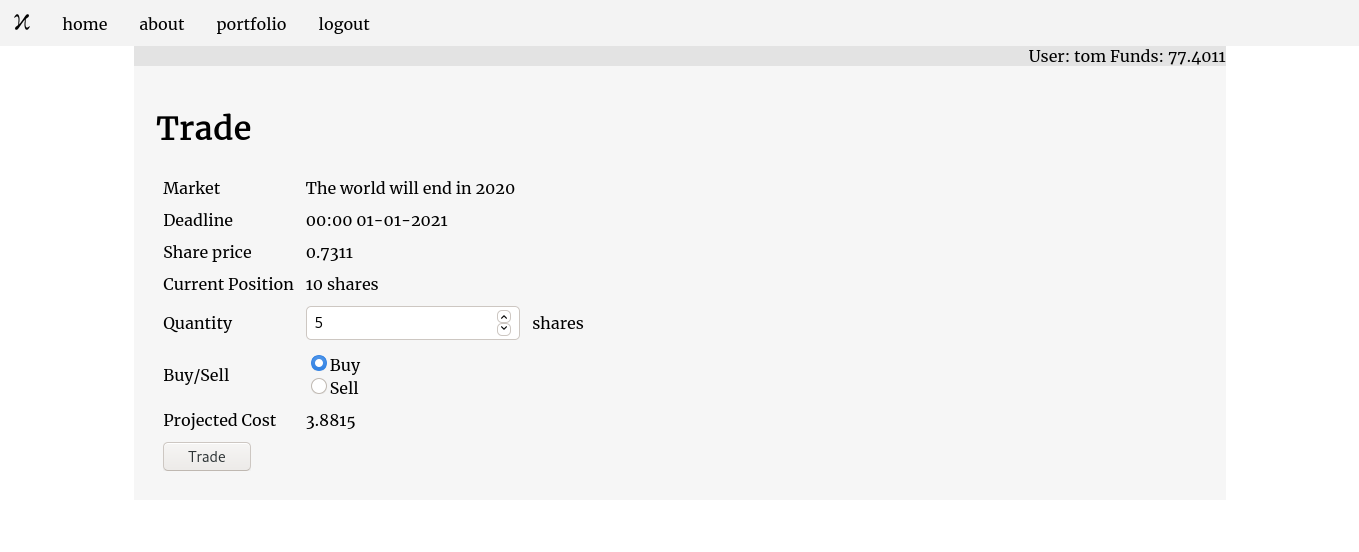
\includegraphics[width=\textwidth]{ajax-price-1}%
	}

	\subfloat[]{%
		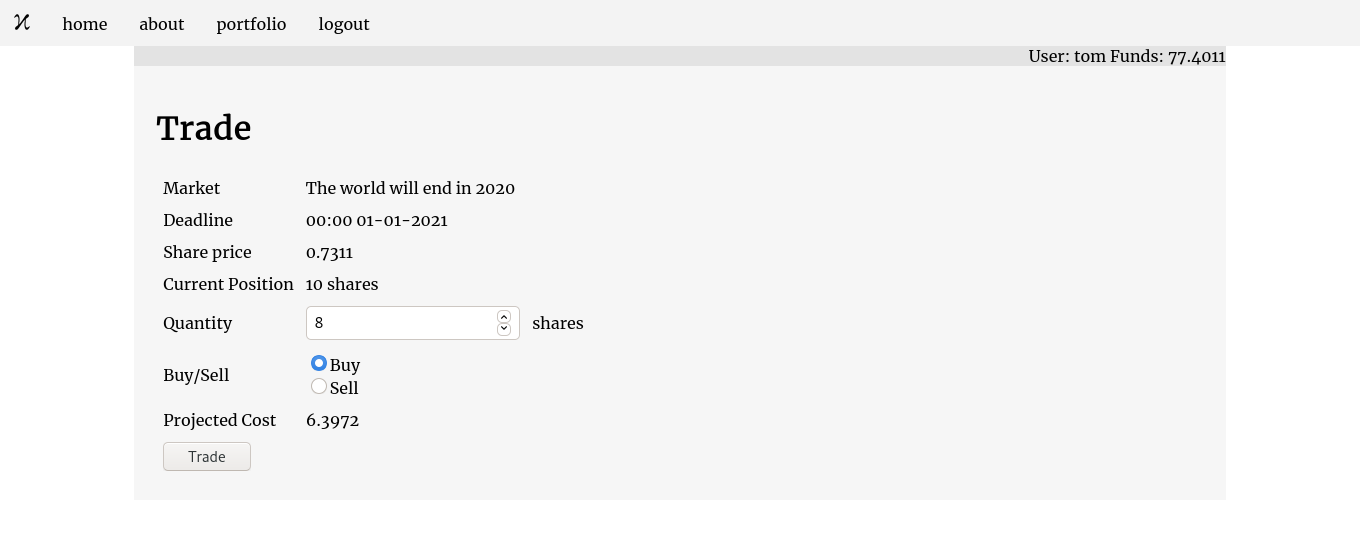
\includegraphics[clip,width=\textwidth]{ajax-price-2}%
	}
	\caption{Updating transaction costs asynchronously}
\end{figure}

\begin{lstlisting}[float,
	label={lst:javascriptTransactionCost},
	caption={Calling the AJAX function asynchronously}]
(ps
  (defun ajax-transaction-cost-trade ()
	" calculate transaction cost when trading in market "
	(let ((quantity (chain document (get-element-by-id :quantity) value))
		  (q (chain document (get-element-by-id :old-shares) value))
		  (radios (chain document (get-elements-by-name "buying")))
		  checked
		  buying-p)

	  ;; find which radio button is checked
	  (loop for option in radios do
			(if (@ option checked)
			  (setf checked (@ option value))))

	  ;; checked is equal to 1 if "buy" is selected
	  (setf buying-p (equal checked 1))

	  (chain smackjack (ajax-transaction-cost-quantity
						 quantity
						 q
						 buying-p
						 display-projected-cost)))))
\end{lstlisting}

Finally, we use AJAX to automatically close trading when a market's deadline
has passed. We first define a Smackjack function that retrieves the most
imminently expiring security, then compute the difference in seconds between
the current time and its deadline. A JSON object is then returned containing
this value, which we use to set a timer for the page to reload. We next define
the Javsacript function \code{set-timer} which takes this JSON object and sets
the page to reload after this interval. This process is given in
Listing~\ref{lst:setTimer}. This prevents user from trading shares after
potentially knowing the outcome, and instead reloads the page and lists the
market under ``Unresolved Markets'' and no longer active (see
Figure~\ref{fig:trade}).

\begin{lstlisting}[float,
	label={lst:setTimer},
	caption={Triggering the close of trading automatically}]
(defun-ajax ajax-set-timer ()
			(*ajax-processor* :method :POST :callback-data :json)

			(let ((next-expiring (db:get-next-expiring-security
								   (local-time:now)))
				  timer)
			  (unless (equal next-expiring NIL)
				(setf timer (local-time:timestamp-difference
							  (db:security-deadline next-expiring)
							  (local-time:now)))
			  (format NIL "{ \"security\" : ~S, \"seconds\" : ~D }"
					  (db:security-bet next-expiring)
					  (ceiling timer)))))

;; within a (:script) tag elsewhere ...
(ps
  (defun set-timer ()
	(chain smackjack
		   (ajax-set-timer #'(lambda (response)
							   (set-timeout (lambda ()
											  (chain location (reload)))
									 		(* (@ response seconds) 1000)))))))
\end{lstlisting}
